
\section{Data Exchange by Example}
The examples in this section show how one can store data for imaging experiments using the Data 
Exchange format. It is general enough, however, to show how Data Exchange can be extended or adapted 
to other techniques. These examples are meant to give a flavor for our approach. A complete reference to 
the core structure can be found in Section \ref{sec:corereference}. Technique specific extensions to the core 
structure can be found at the end of the Reference Guide.

\subsection{Diagram color code}
All the diagrams in this section follow the color conventions shown in Figure \ref{fig:DiagramColorCode}. 
The basic elements are HDF5 datasets, attributes, and groups. We also support internal references to 
elements in the file by a simple scalar string that holds the path of the dataset within the file. On the 
diagram, this is shown as a reference dataset that points to the referred-to dataset. Note that we use this 
mechanism rather than HDF5 hard or soft links
\label{DiagramColorCode}

\begin{figure}[h!]
\centering
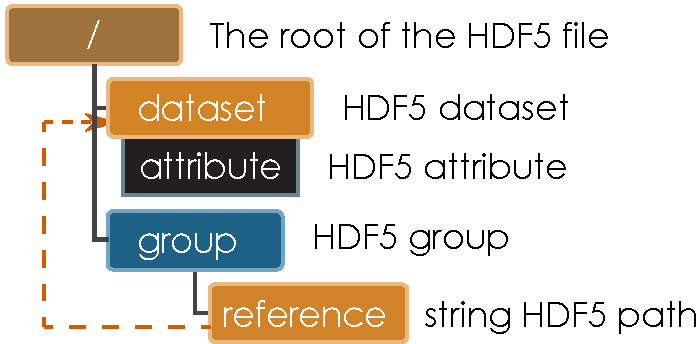
\includegraphics[width=0.5\textwidth]{figures/dx_DiagramColorCode.pdf}
\caption{Explanation of the color code used in the diagrams}
\label{fig:DiagramColorCode}
\end{figure}

\subsection{A minimal Data Exchange file for imaging}
Figures \ref{fig:Minimal1} shows a diagram of a minimal Data Exchange file to store a single projection 
image.  It is strongly encouraged that all datasets shall have a units attribute. The axes of the dataset are 
not specified in this minimal
case, and can be assumed to be x and y with a zero-based integer sequence, or more simply, pixels.
 
\begin{figure}[h!]
\centering
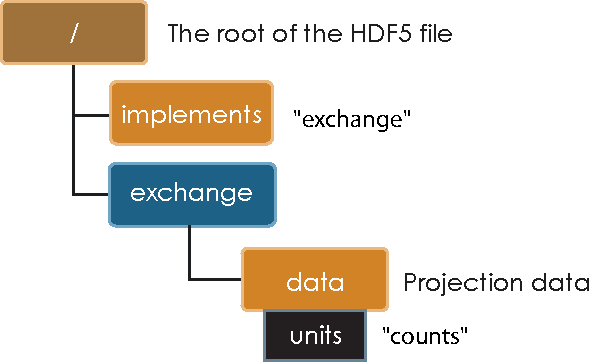
\includegraphics[width=0.5\textwidth]{figures/dx_Minimal1.pdf}
\caption{Diagram of a minimal Data Exchange file for a single image.}
\label{fig:Minimal1}
\end{figure}

\subsection{Storing and describing a multidimensional dataset}
A multidimensional dataset should be described as fully as possible, with units for the dataset as well as 
dimension descriptors (that also have units defined). There are also additional descriptive fields available 
such as title and description. The order of dimensions in the dataset should put the slowest changing 
dimension first, and the fastest changing dimension last. 

It is strongly encouraged that all datasets have a units attribute. The string value for units should preferably 
be an SI unit, however well understood non-SI units are acceptable, in particular "degrees". The units 
strings should conform to those defined by UDUNITS at {http://www.unidata.ucar.edu/software/udunits}. 
While UDUNITS is a software package, it contains simple XML files that describe units strings and 
acceptable aliases.

The axes of a multidimensional dataset are described through the use of additional one-dimensional 
datasets (dimension descriptors), one for each axis in the main dataset. Take for example a 3-dimensional 
cube of images, with axes of x, y, and z where z represents the angle of the sample when each image was 
taken. There should be 3 additional one-dimensional datasets called x, y, and z where x and y contain an 
integer sequence, and z contains a list of angles. X and y have units of "counts" and z has units of 
"degrees". To simplify, it is acceptable to omit x and y, since the default interpretation will always be an 
integer sequence. 

The dimension descriptors (x, y, and z) can be associated with the main dataset through two mechanisms. 
The HDF5 libraries contain a function call H5DSattach\_scale to "attach" a dimension descriptor 
dataset to a given dimension of 
the main dataset. HDF5 takes care of entering several attributes in the file that serve to keep track of this 
association. If the particular programming language you work in does not support this HDF5 function, then 
you can instead add a string attribute to your main dataset called axes. The axes attribute is simply a colon 
separated string naming the dimension descriptor datasets in order, so "z:y:x" in this case. Additional 
examples below show this in action.

\subsection{Storing projections, dark fields, and white fields}
\label{section:minimalTomo}

A tomographic data set consists of a series of projections, dark and white field images. The dark and white fields must have the same projection image dimensions and can be collected at any time before, after or during the projection data collection. The angular position of the tomographic rotation axis, theta, can be used to keep track of when the dark and white images are collected.  These examples show projection, dark, and white images saved in three 3D arrays as shown in Figure \ref{fig:MinimalTomo0} and \ref{fig:MinimalTomo1} using, by default, the natural HDF5 order of the a multidimensional array (rotation axis, ccd y, ccd x), i.e. with the fastest changing dimension being the last dimension, and the slowest changing dimension being the first dimension. If using the default dimension order, the axes attribute "theta:y:x" can be omitted. The {\tt{axes}} attribute is mandatory if the 3D arrays use a different axes order. This could be the case when, for example, the arrays are optimized for sinogram read ({\tt{axes}} = "y:theta:x"). As no units are specified the data is assumed to be in ``counts'' with the axes (x, y) in pixels. 

If the positions of the rotation axis for each projection, dark, and white images are not specified via theta dimension scale datasets, it is assumed that the raw projections are taken at equally spaced angular intervals between 0 and 180 degree, with white and dark field collected at the same time before or after the projection data collection.

\begin{figure}[h!]
\centering
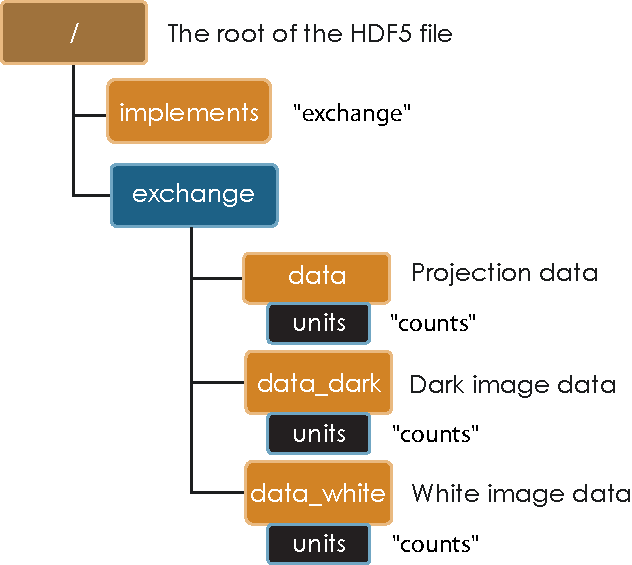
\includegraphics[width=0.5\textwidth]{figures/dx_MinimalTomo0.pdf}
\caption{Diagram of a minimal Data Exchange file for a single tomographic data set including raw projections, dark, and white fields.}
\label{fig:MinimalTomo0}
\end{figure}

\begin{figure}[h!]
\centering
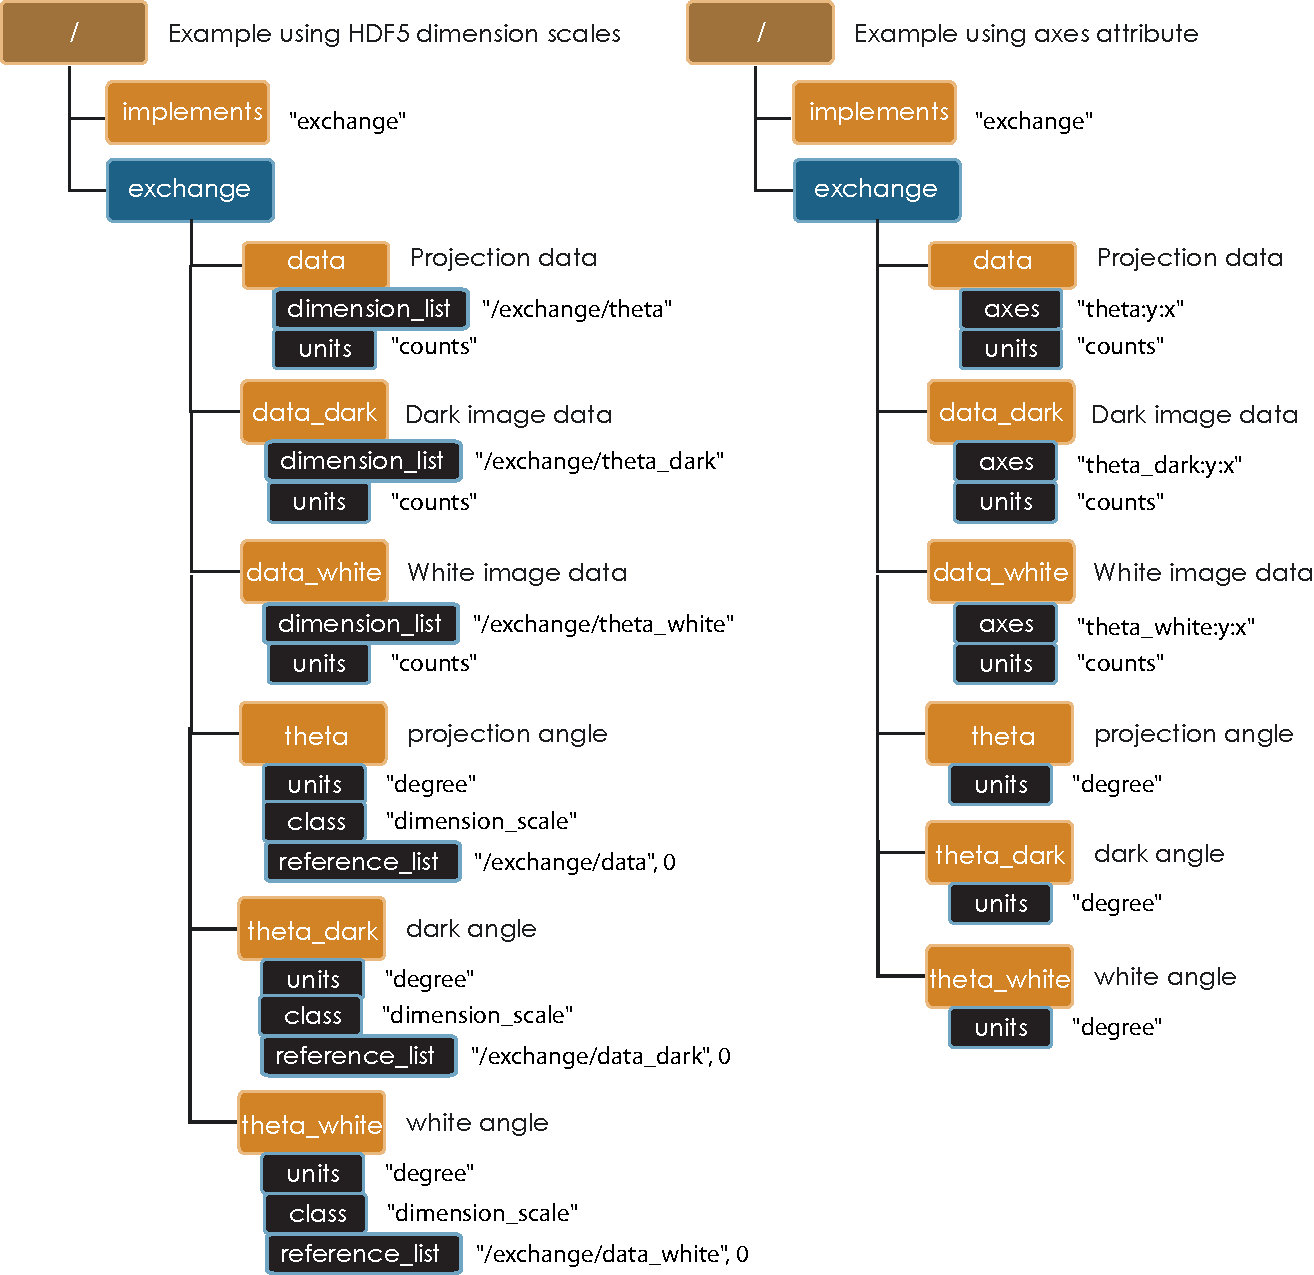
\includegraphics[width=0.8\textwidth]{figures/dx_MinimalTomo1.pdf}
\caption{Diagram of a single tomographic data set including raw 
projections, dark and white fields. In this case, there are additional dimension descriptor
datasets theta, theta\_dark, and theta\_white that contain the positions of the rotation axis
for each projection, dark, and white image. The lefthand example shows this as it would
appear using the HDF5 H5DSattach\_scale function. The righthand example shows this as it would
appear by manually adding an axes attribute (for cases where H5DSattach\_scale is unavailable).}


\label{fig:MinimalTomo1}
\end{figure}

\subsection{A typical Data Exchange file for tomography}
A series of tomographic data sets are typically collected changing the instrument status (energy, detector or 
optics position) or changing the sample status (position, environment etc.). Figure \ref{fig:MinimalTomo2}, 
\ref{fig:MinimalTomo3} and \ref{fig:MinimalTomo4}  show the content of files changing the sample 
temperature, the x-ray source energy and detector-sample distance. 

\subsubsection{Sample Temperature Scan}
\begin{figure}[h!]
\centering
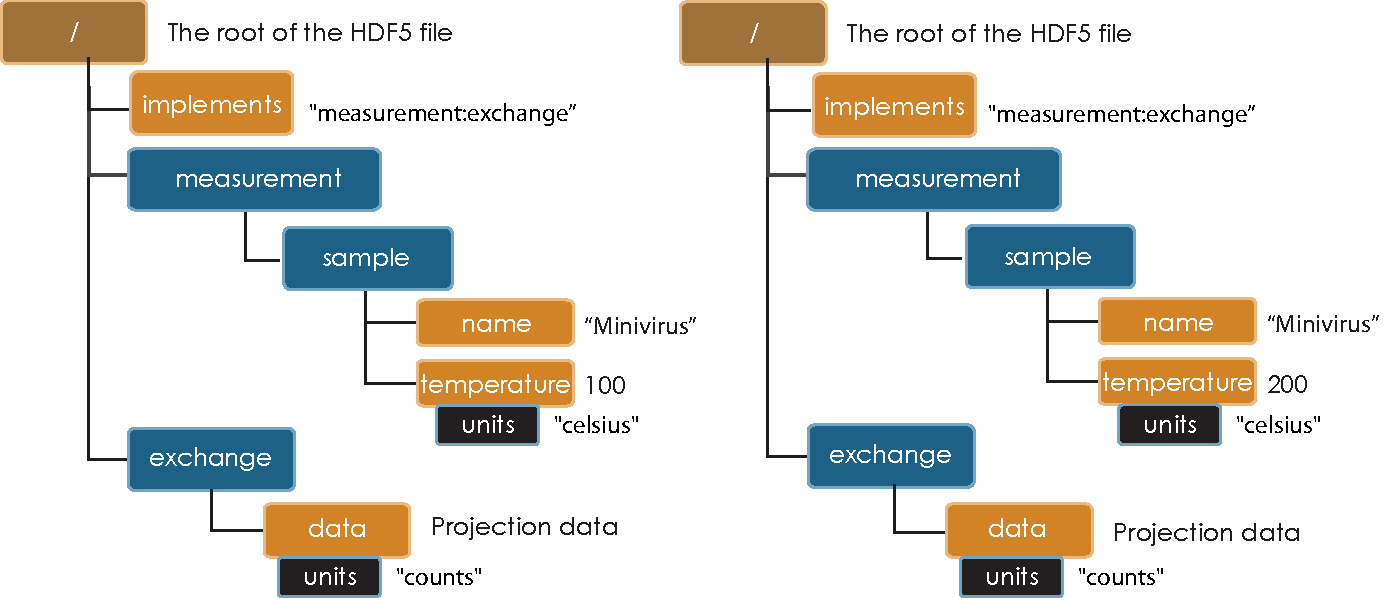
\includegraphics[width=1.0\textwidth]{figures/dx_MinimalTomo2.pdf}
\caption{Diagram of two tomographic data sets taken at two different sample temperatures (100 and 200 celsius).}
\label{fig:MinimalTomo2}
\end{figure}

\clearpage
\subsubsection{X-ray Energy Scan}
\begin{figure}[h!]
\centering
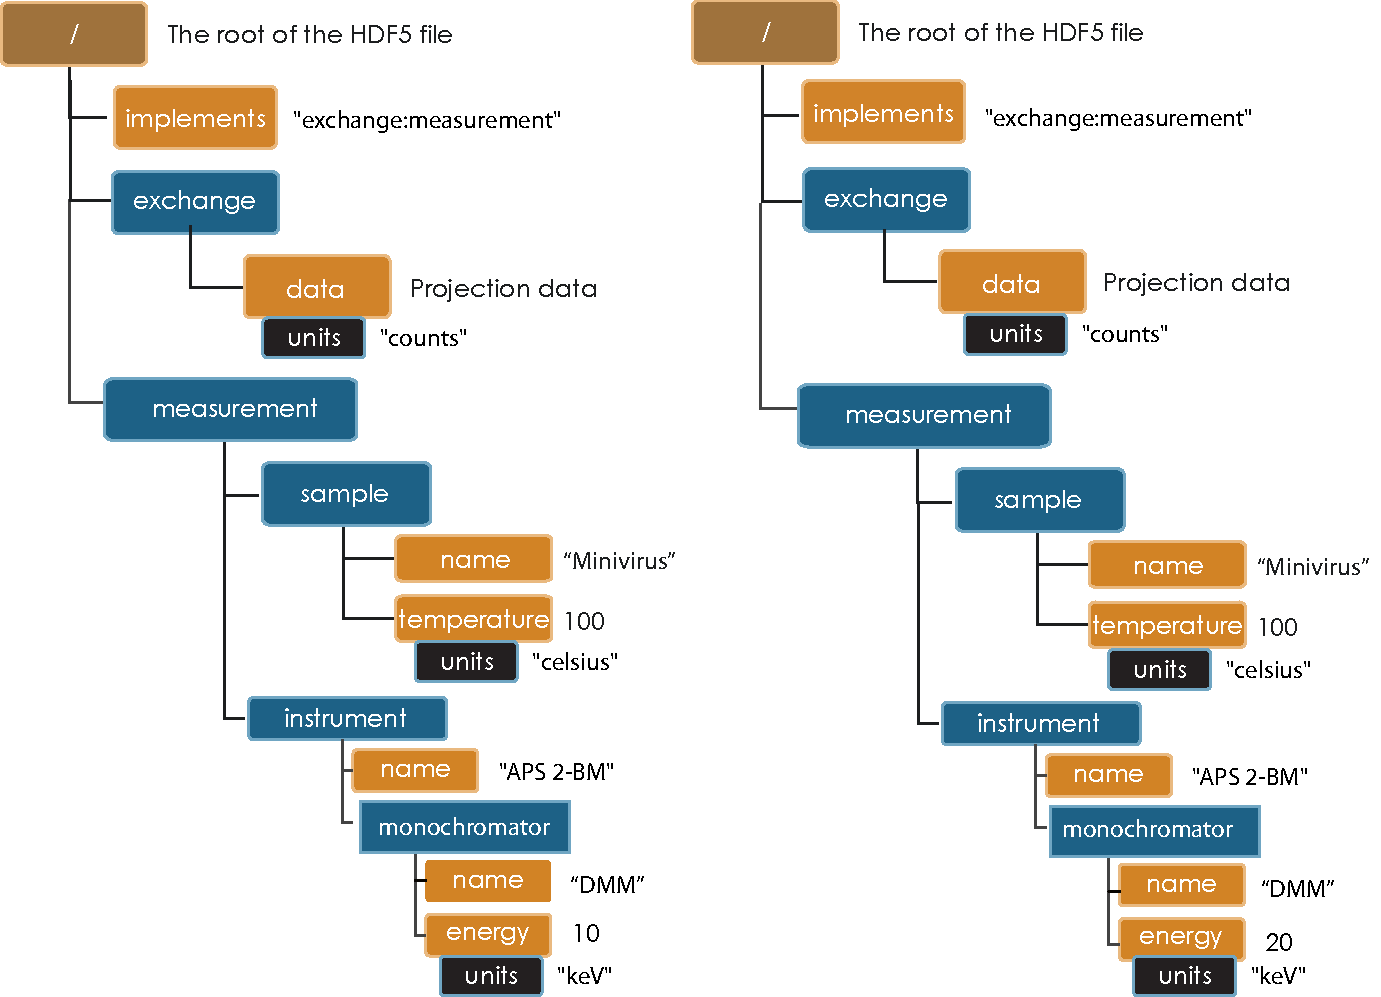
\includegraphics[width=0.8\textwidth]{figures/dx_MinimalTomo3.pdf}
\caption{Diagram of two tomographic data sets taken at two different energy (10 and 20 keV).}
\label{fig:MinimalTomo3}
\end{figure}

\clearpage
\subsubsection{Detector-sample Distance Scan}
\begin{figure}[h!]
\centering
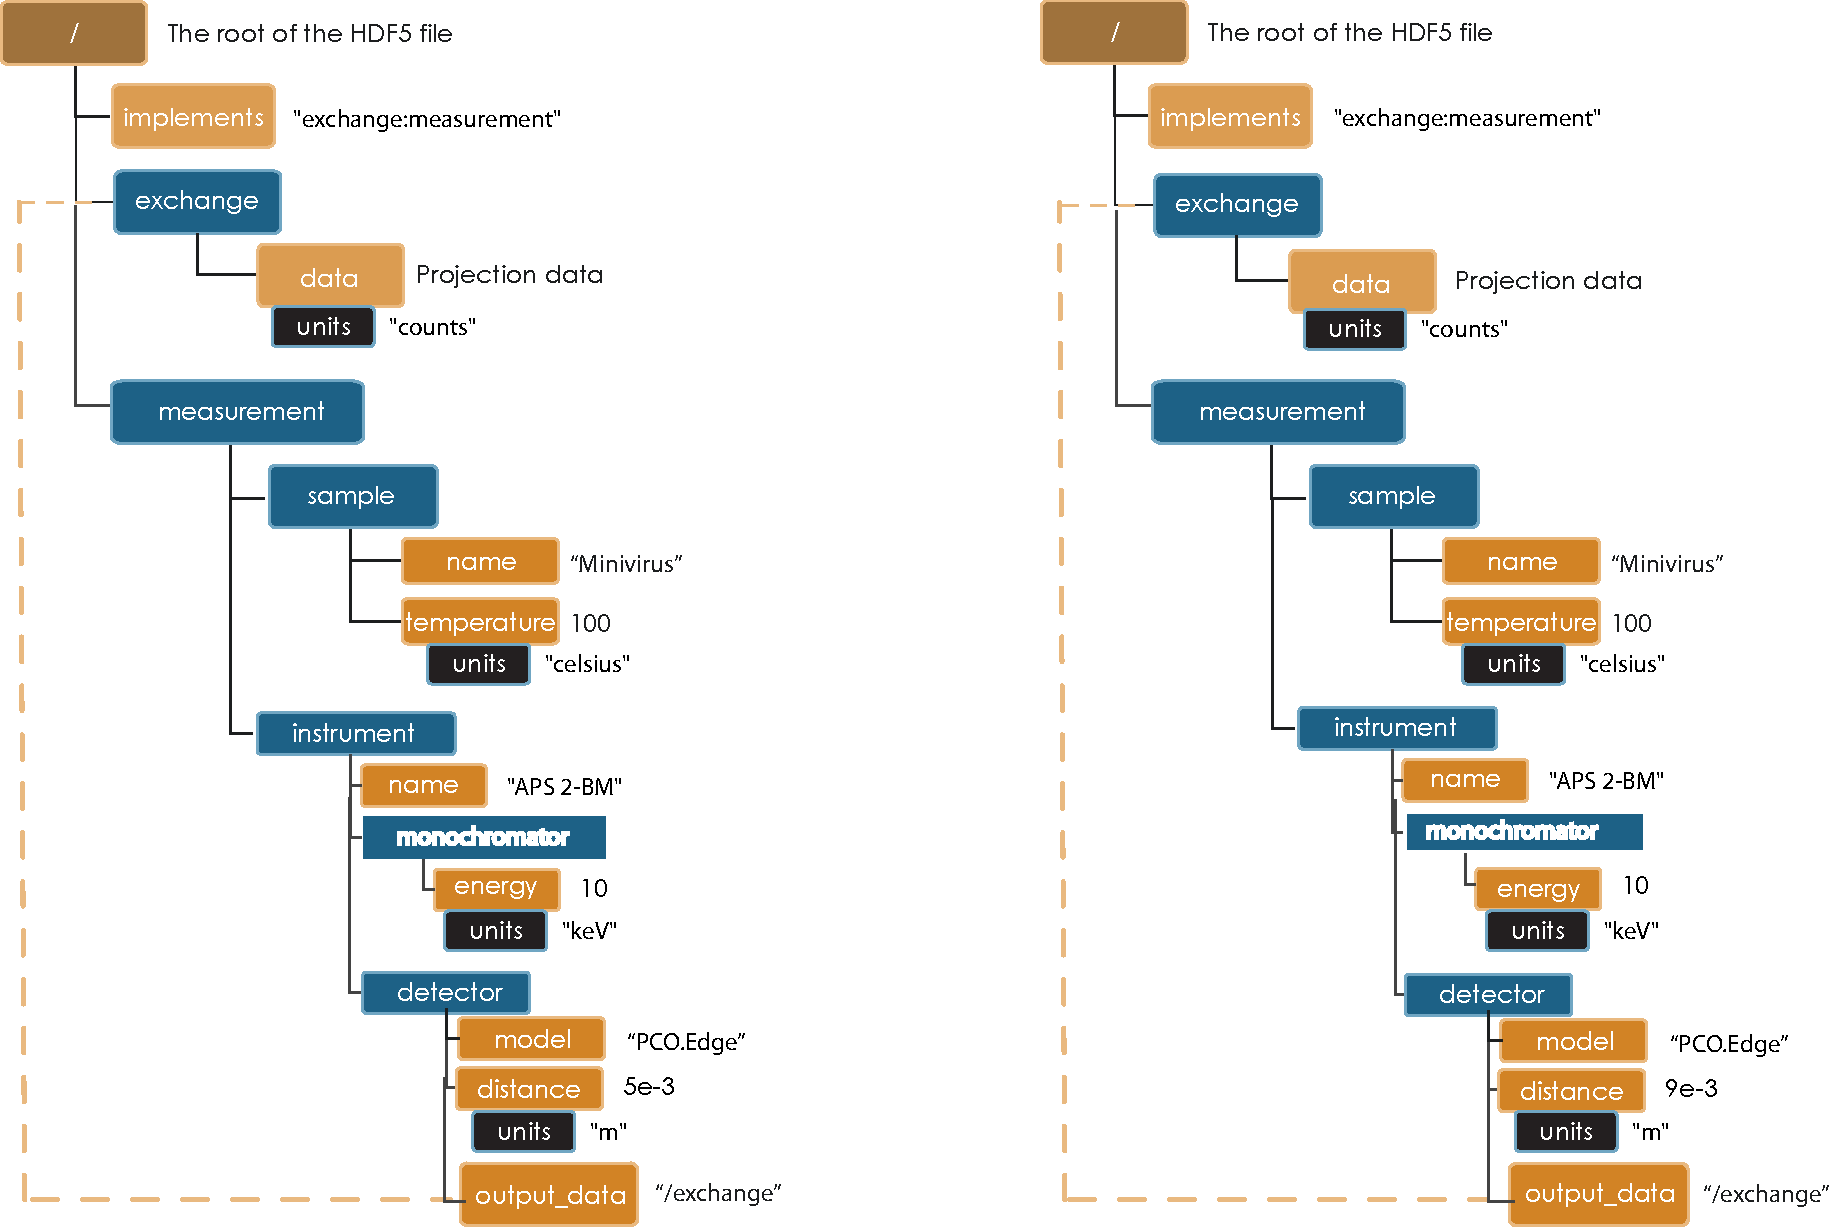
\includegraphics[width=0.8\textwidth]{figures/dx_MinimalTomo4.pdf}
\caption{Diagram of two tomographic data sets collected with two different detector-sample distances (5 and 9 mm). Note the use of {\tt output\_data} dataset to associate the detector with the exchange group generated from the acquisition.}
\label{fig:MinimalTomo4}
\end{figure}

\subsubsection{Series of Tomographic Measurements}

A series of tomographic measurements, when relevant, can be stored in the same file appending \_$N$ to the measurement tag. In nano tomography experiments, for example, the detector field of view is often smaller than the sample. To collect a complete tomographic data set, it is necessary to raster the sample across the field of view moving its x and y location. Figure \ref{fig:NanoTomo1}  shows a file from a nano tomography experiment when the sample rasters through the field of view.  

There are limits to this approach, as one clearly does not want to have hundreds of measurement groups in a file (or multiple files) where most of the metadata is the same. For measurements where there are many "positioner" values (aka a "scan"), it is more sensible to add dimension(s) to the exchange dataset, and describe the "positioner" values as dimension scales. This is a judgement left to the user.

\begin{figure}[h!]
\centering
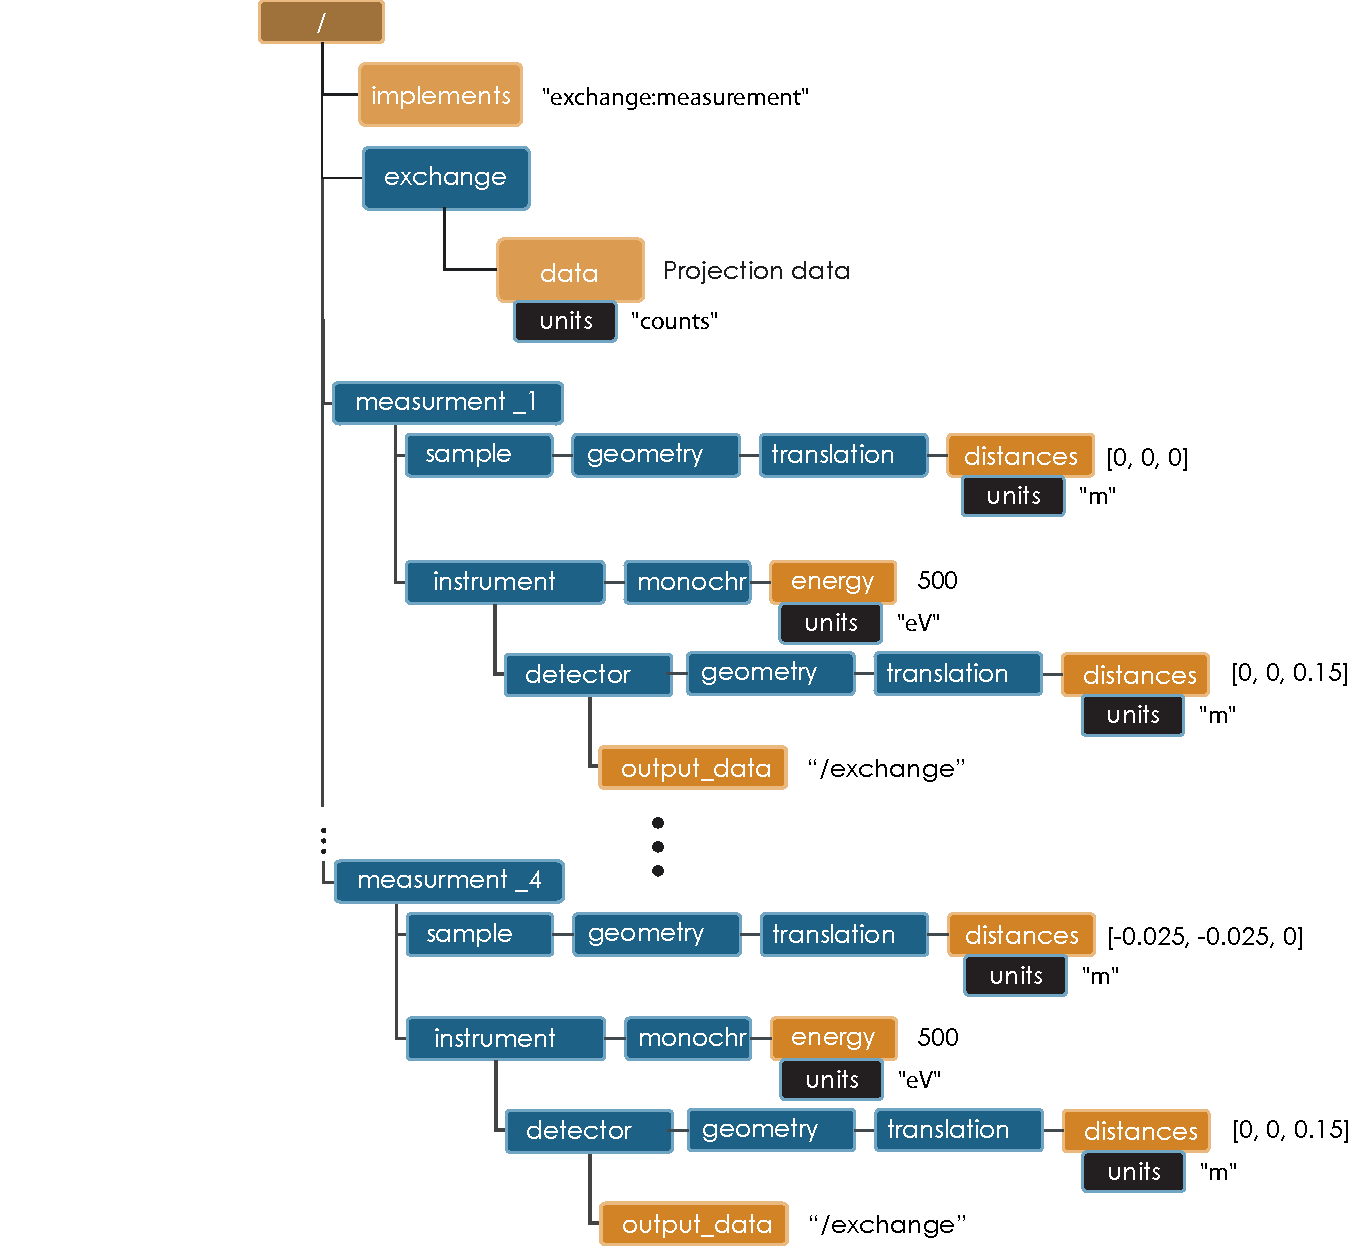
\includegraphics[width=0.9\textwidth]{figures/dx_NanoTomo1.pdf}
\caption{Diagram of a file with 4 tomographic data sets from a nano tomography experiment.}
\label{fig:NanoTomo1}
\end{figure}
